\documentclass[largeformat]{interact}
\usepackage{fontspec}
\setmainfont{Noto Serif}
\setsansfont{Noto Sans}
\usepackage{unicode-math}
\setmathfont{Latin Modern Math}
\let\eth\relax
\usepackage{amsmath}
\usepackage{natbib}
\bibpunct[, ]{(}{)}{;}{a}{}{,}
\renewcommand\bibfont{\fontsize{10}{12}\selectfont}
\usepackage{longtable,booktabs,array}
\usepackage{calc}
\usepackage{enumitem}
\usepackage{microtype}
\usepackage{xurl}
\usepackage[hidelinks]{hyperref}
\usepackage{bookmark}
\setlength{\parindent}{0pt}
\setlength{\parskip}{4pt plus 1pt minus 1pt}
\setlength{\emergencystretch}{2em}
\setlength{\tabcolsep}{3pt}
\renewcommand{\arraystretch}{1.13}
\setlength{\LTleft}{0pt}
\setlength{\LTright}{0pt}
\providecommand{\tightlist}{\setlength{\itemsep}{0pt}\setlength{\parskip}{0pt}}
\hypersetup{pdftitle={RFNBO Price Pathways and Renewable Hydrogen Plant Design: An Origin Aware Engineering Study of Selected European Market Areas},pdfauthor={Junjie Zhang},pdfsubject={International Journal of Green Energy -- Original article}}
\begin{document}
\articletype{ORIGINAL ARTICLE}
\title{RFNBO Price Pathways and Renewable Hydrogen Plant Design: An Origin Aware Engineering Study of Selected European Market Areas}
\author{
\name{Junjie Zhang\textsuperscript{a,b}\thanks{CONTACT Junjie Zhang. Email: \href{mailto:junjiezhang2024@shisu.edu.cn}{junjiezhang2024@shisu.edu.cn}; ORCID: \href{https://orcid.org/0009-0004-8821-4018}{0009-0004-8821-4018}}}
\affil{\textsuperscript{a}Shanghai Academy of Global Governance \& Area Studies, Shanghai International Studies University, Shanghai 201620, China; \textsuperscript{b}School of Economics and Finance, Shanghai International Studies University, Shanghai 201620, China}
}
\maketitle

\begin{abstract}
Renewable hydrogen plants balance renewable capacity, storage, and grid electricity admitted by a price pathway. We develop an origin aware linear program that preserves electricity provenance in battery and hydrogen storage. Across 18 European cells, profile shifts change modeled savings by a median 0.82 percentage points and up to 4.86 points. The 2019 median saving is 1.31\%; 16 of 18 cells are below 3\%, while SK reaches 11.77\% and EE has no response. Value therefore depends on temporal coincidence, not trigger frequency alone. This is an engineering screen, not legal certification or an EU 27 network estimate.
\end{abstract}

\noindent\textit{Word count: 6,279}

\section{Introduction}\label{introduction}

Renewable hydrogen projects must choose whether to meet a delivery
target mainly by building renewable capacity and storage or by using
permitted grid electricity during qualifying hours. That choice changes
the optimal mix of wind, solar, electrolyzer capacity, storage, and
imported electricity. The delegated regulation for renewable fuels of
non biological origin (RFNBO) places temporal, geographical, and
additionality conditions around electricity sourcing, while its price
pathway gives a narrow route for treating grid electricity as renewable
under specified conditions \citep{ref25,ref26}. The engineering
consequence is a design problem: under an explicit rule proxy, when can
qualifying grid imports replace costly renewable overbuild or storage,
and when does the least cost design remain unchanged?

The central engineering uncertainty is whether eligible price hours
arrive when the renewable only design is short of renewable supply; a
high trigger count alone need not create a capacity margin.

Existing European studies establish why the question matters. Brandt et
al.~assess the cost and competitiveness consequences of the European
regulatory framework \citep{ref01}. Ruhnau and Schiele evaluate how
relaxing simultaneity changes hydrogen project design, economics, and
power sector emissions \citep{ref02}. Zeyen et al.~examine temporal
regulation of renewable supply, while Namazifard et al.~compare
unrestricted and green electrolytic hydrogen under EU criteria
\citep{ref03,ref04}. Studies of portfolio effects, PPAs, carbon
accounting incentives, and spatial design extend the discussion to
system, contractual, or European wide settings
\citep{ref05,ref06,ref07,ref08,ref16,ref17,ref18,ref20}. Complementary
project studies analyze curtailment, active trading, renewable
configurations, and temporal correlation
\citep{ref09,ref10,ref15,ref21,ref22}. Recent preprints also address
cost upper bounds, PPA uncertainty, exporters, and market participation
\citep{ref11,ref12,ref23,ref24}.

Three features of that literature sharpen the present question. First,
system wide studies appropriately optimize electricity sector
interactions or emissions but do not necessarily identify the project
boundary capacity substitutions that a price pathway proxy enables.
Second, studies that relax temporal matching show that timing matters,
yet a comparison of relaxed rules alone does not reveal whether the
frequency of eligible price hours or their alignment with a plant's
renewable profile creates the economic margin. Third, models that
combine electricity and hydrogen storage can produce different designs
depending on whether energy provenance is retained after charging. For a
rule sensitive plant sizing exercise, allowing a grid origin charge to
inherit renewable provenance would change the accounting problem itself.
The practical gap is therefore not another map of average hydrogen cost:
it is a transparent test of which timing and accounting conditions turn
an expanded rule pathway into a material design difference.

Existing studies establish that timing and regulatory design matter for
hydrogen costs and emissions \citep{ref01,ref02,ref03,ref04}. Three
engineering questions remain. First, how large is the design response
when the price pathway is isolated from other regulatory elements?
Second, is the response driven by eligible hour frequency or by temporal
coincidence between low price hours and renewable output? Third, does
the response transfer across years, public profiles, and bounded
technology assumptions? These are plant design mechanism questions
rather than system cost questions. They require origin preserving
storage accounting and a temporal phase shift experiment, which we
implement in a common linear programming framework.

This study therefore asks three engineering questions. \textbf{RQ1:}
Under an origin aware price pathway proxy, how large are the LCOH and
capacity differences from the renewable only baseline in a selected
public data screen? \textbf{RQ2:} Holding price traces, EUA values,
trigger frequency, delivery target, and engineering caps fixed, does
changing only the timing of wind and solar profiles materially change
those differences? \textbf{RQ3:} Do the magnitude, branch attribution,
and capacity response transfer across retained years, public published
day ahead profiles, and bounded technology cost assumptions?

The paper's differentiating contribution is an auditable, reproducible,
conditional engineering comparison. It integrates origin tagged storage
accounting and price branch decomposition in a single linear program,
proves the nested feasible set property that separates structural
direction from empirical magnitude, and evaluates a predeclared temporal
shift mechanism, cross period/profile sensitivity, and finite parameter
stress. The estimand is the difference in least cost model boundary LCOH
and asset capacity for selected, separately solved public data market
area/profile cells. This design makes the timing mechanism and its
capacity consequences inspectable without treating a local response as a
European wide property.

The scope is fixed at the estimand level. This is a public data
engineering screening study. The estimand is the conditional difference
in least cost model boundary LCOH and asset capacity for selected,
separately solved public market area/profile cells. Legal RFNBO
certification, including complete additionality, geographical
correlation, contracting, metering, support, and production evidence, is
outside the estimand. The study also does not estimate EU-27 project
level prevalence, project level congestion, bidding zone congestion,
point forecasts, authenticated forecast vintage performance, real time
operation, or site specific interconnection, metering, and contract
outcomes. Within this boundary, the model preserves renewable and grid
provenance in separate storage ledgers and uses controlled timing, cross
period, and bounded parameter comparisons to identify conditional design
responses.

\section{Materials and methods}\label{materials-and-methods}

\subsection{Study boundary and research
design}\label{study-boundary-and-research-design}

The study is a selected European public data engineering screen. The
primary layer has 18 complete 2019 cells, each pairing a public
wind/solar generation shape with a public day ahead price area. DE-LU is
represented as its coupled market area; DK1 and IT North are paired with
country level renewable profile shapes. These cells were retained for
complete paired hourly data and profile diversity, not sampled
probabilistically from projects or EU bidding zones. We selected 2019 as
the primary screen because it provides a before the COVID 19 pandemic
historical benchmark with the common paired hourly coverage retained
across all 18 cells; E2 tests transfer to later years and alternative
published profiles. Each cell has a fixed annual hydrogen delivery
target, scaled to retained UTC hours, a 250 MW source line proxy, and a
1,000 MW grid import proxy. The model compares a renewable only baseline
with declared computational price pathway cases at the same target and
cost boundary.

The analysis is interpreted within this declared study boundary. The
2019 hourly traces serve as a historical engineering stress test of a
2030 rule representation and are used comparatively rather than as 2030
price forecasts.

Table 1 summarizes the predeclared evidence sequence.




\subsection{Rule proxy and nested feasible
sets}\label{rule-proxy-and-nested-feasible-sets}

The model implements a computational price pathway proxy. In hour \(t\),
the low price indicator is

\[
I_t=\mathbb{1}\{p_t\leq20\ \text{EUR/MWh}\ \lor\ p_t<0.36E_t\},
\]

where \(p_t\) is the day ahead price and \(E_t\) is the daily EUA
auction price carried across the corresponding UTC day. The
implementation separately solves negative price only, EUR 20/MWh only,
EUA only, joint, and renewable only cases when the experiment calls for
branch decomposition. The EUR 20/MWh threshold represents the low price
branch encoded by the RFNBO rule proxy, whereas \(0.36E_t\) is the
declared computational signal used for the EUA linked branch. The latter
is not treated as legal equivalence. Hereafter, ``price pathway proxy''
denotes the rule representation, and ``model qualified grid
electricity'' denotes grid energy admitted by that proxy and selected by
the optimization; neither phrase is a legal certification. The indicator
is a transparent computational signal, while legal certification and
site evidence questions remain outside the estimand. This separation
makes the price logic explicit so it can be stress tested reproducibly.

The direction of the price pathway comparison has a simple structural
property. Let \(\mathcal{F}_R\) be the renewable only feasible set and
\(\mathcal{F}_P\) the price pathway feasible set. A renewable only
solution remains feasible under the price pathway formulation by setting
all model qualified grid flows and all grid origin storage flows to
zero. All remaining balances and the delivery target are unchanged. Thus
\(\mathcal{F}_R\subseteq\mathcal{F}_P\). With the same objective, the
optimized costs obey \(J_P\leq J_R\). Nonnegative modeled savings
therefore follow from the formulation.

\textbf{What the model identifies.} Because the feasible sets are
nested, cost direction is structural rather than empirical. The
empirical contribution begins with three quantities that are not
structural: (i) the magnitude of strict savings, which indicates whether
the pathway is materially useful in a cell; (ii) the capacity
substitution pattern, which identifies the renewable or conversion
assets the optimizer avoids; and (iii) the response to controlled timing
shifts, which tests how temporal coincidence changes the substitution
margin. Each quantity is conditional on the public profile, price trace,
delivery target, and declared cost box. This is the basis for
interpreting the results below.

\subsection{Origin aware linear
program}\label{origin-aware-linear-program}

For each cell, the linear program chooses wind capacity \(K_W\), solar
capacity \(K_S\), battery power and energy \((K_B,E_B)\), electrolyzer
capacity \(K_E\), hydrogen storage \(K_H\), and hourly
electricity/hydrogen flows. It minimizes annualized capacity cost plus
variable electricity, grid fee, and battery degradation cost:

\[
\min_{K,x} J=\sum_i a_i c_iK_i+\sum_t\Delta t\left[(p_t+f_g)g_t+c_Bb_t\right],
\]

where \(a_i c_i\) is the annualized unit cost of asset \(i\), \(g_t\) is
grid import, \(f_g\) is the declared grid fee, and \(b_t\) is battery
throughput. Screening LCOH is \(J\) divided by the fixed delivered
hydrogen quantity. The objective includes wind, solar, battery,
electrolyzer, hydrogen storage, declared electricity, grid fee, and
degradation terms. It excludes water, compression, transport, taxes,
financing, lifecycle inventories, project development, and offtake
costs.

Under the central cost vector, the optimizer selects zero battery
capacity in all 18 primary price pathway solutions. We do not impose
this outcome. It follows from the joint interaction of annualized asset
costs, conversion efficiencies, storage losses, and hourly operating
costs; E3 tests how the resulting cost and capacity response changes
within the bounded parameter box.

Renewable availability is bounded by \(K_WCF^W_t+K_SCF^S_t\), and source
line and grid import limits constrain hourly flows. Renewable- and grid
origin battery inventories are separate. Renewable origin and non
renewable hydrogen inventories are also separate. In the model qualified
route, electrolyzer load credited by the model is balanced only by
renewable direct flow, renewable tagged battery discharge, and
qualifying grid input. Terminal storage states are zero, which prevents
endpoint energy from reducing the objective artificially. A cumulative
renewable energy safeguard restricts model qualified grid energy to no
more than optimized renewable generation over the represented horizon.
This is a conservative quantity surrogate, not a complete Article 5
(RFNBO additionality) legal test.

This accounting structure makes the comparison interpretable. Direct
renewable electricity, renewable electricity discharged from the
battery, and model qualified grid electricity are mutually identified in
every represented hour. Grid origin battery energy remains in its own
ledger and cannot support model qualified hydrogen delivery. The annual
quantity safeguard is applied after hourly balances rather than
substituted for them; it cannot create qualifying electricity in an hour
that fails the price indicator. Conversely, a low price hour does not
force grid import: the optimizer uses it only if it reduces the declared
total cost while meeting the same delivery target and all source line
limits. This distinction matters for interpreting a capacity response. A
reduction in solar or electrolyzer capacity is not assigned mechanically
by the rule; it is an optimized substitution that occurs only when the
timing, price, and capacity constraints make it less costly than
renewable overbuild.

The complete code aligned balance equations, bounds, and variable
definitions are supplied in the reproducibility package. The main text
presents the governing objective and accounting logic because the
storage provenance control is central: a grid import cannot
retrospectively turn renewable storage into grid origin energy, and a
renewable charge cannot be counted twice.

\subsection{Public data, processing, and
reproducibility}\label{public-data-processing-and-reproducibility}

The primary 2019 generation profiles use the Energy-Charts public API
and country generation series \citep{ref39,ref44}. Primary day ahead
price series use the public archived ENTSO-E-derived snapshot with its
recorded dataset DOI \citep{ref45}. Cross period DE-LU price and
generation series use publicly accessible Energy-Charts/SMARD sources,
while Belgian observed and published day ahead profile series use Elia
public data \citep{ref40,ref41}. EUA prices are drawn from public EEX
market data \citep{ref34}. Technology assumptions are declared from the
Danish Energy Agency technology data source and fixed engineering
parameters \citep{ref35}. Area identifiers and access conventions follow
ENTSO-E public documentation \citep{ref27,ref28}.

The public data requirement is a design constraint rather than a
rhetorical feature. The analysis uses no private plant dispatch,
confidential connection agreement, proprietary forecast archive, or paid
market database. Each derived cache records a source path, UTC coverage,
transformation manifest, and SHA-256 digest. A source is retained only
when the paired hourly fields required by its experiment are available
under the documented public access route. This produces a narrower
estimand than a project study, but it permits an independent researcher
to inspect the inputs and rerun the comparison without a commercial data
license or an operator partnership.

All model timestamps are UTC. Retained primary cells contain 8,687 to
8,760 paired hours, and no missing hour is imputed. E2 retains every
planned source year profile with at least 99\% complete hours; the
achieved minimum was 99.726\%. Local calendars select years only;
daylight saving transitions are represented through the underlying UTC
hour sequence. The Belgian published day ahead profiles do not carry an
authenticated issue time field in the retained public source. They are
therefore a public published profile sensitivity only, not forecast
vintage validation, real time evidence, or a forecast error estimate.

The base cost vector is fixed before the experiments: 120,000
EUR/MW/year for wind, 85,000 EUR/MW/year for solar, 45,000 EUR/MW/year
for battery power, 12,000 EUR/MWh/year for battery energy, 100,000
EUR/MW/year for the electrolyzer, and 2 EUR/kg/year for hydrogen
storage. Renewable variable cost is 1 EUR/MWh, the base grid fee is 3
EUR/MWh, and battery degradation is 2 EUR/MWh. The base hydrogen yield
is 20 kg/MWh; charge and discharge efficiencies are 0.90 for the battery
and 0.995 for hydrogen. These are annualized engineering assumptions,
not observed project quotations. E3 varies the declared grid fee and
other bounded assumptions around this same reference configuration.




The derived public data cache, scenario manifest, solver checks,
numerical claim ledger, code hash inventory, and editable result tables
were stored in the reproducibility package used for this manuscript. The
package contains the transformation record and the public source
identifiers needed to inspect the reported calculations; no
authenticated credential or private dataset is used.

\subsection{Experiments and technical
checks}\label{experiments-and-technical-checks}

\textbf{E1: temporal phase shift.} For every primary cell, wind and
solar curves were jointly circularly shifted by 0, 2,190, 4,380, and
6,570 retained hourly positions. Prices, EUA values, rule trigger
counts, delivery target, costs, and engineering caps were fixed. This is
a synthetic timing perturbation, not a realized operating case. It
isolates temporal coincidence while keeping each cell's price
distribution and trigger frequency unchanged.

\textbf{E2: cross period and public published profile sensitivity.} We
solved five cases (renewable only, negative only, EUR 20/MWh only, EUA
only, and joint) for DE-LU observed 2019-2022; BE observed 2021-2025;
and BE published day ahead profiles for 2021-2025. All source year
profiles meeting the prespecified completeness criterion were retained.
The comparison asks whether branch attribution and magnitude change
across public hourly curves, rather than treating one historical year as
general.

\textbf{E3: bounded parameter stress.} The 18 primary cells were run
under the base parameterization plus 12 fixed seed Latin hypercube
draws. The finite stress box varies CAPEX by 0.80-1.20, hydrogen yield
by 0.90-1.10, grid fee from 0-6 EUR/MWh, battery charge/discharge
efficiency from 0.85-0.95, hydrogen charge/discharge efficiency from
0.98-1.00, and the EUA proxy by 0.80-1.20. These are engineering ranges,
not distributions. Consequently, ranges reported below are neither
confidence intervals nor probability statements.

The audit required every solver status to equal zero, delivery target
error below 1e-4 kg, electricity/source line/eligible grid excess below
1e-5 MW, zero terminal storage states, strictly UTC timestamps, valid
cache hashes, and complete planned scenario coverage. The phase shift
zero position reproduced the pre upgrade primary baseline and joint LCOH
values to a maximum absolute error of 0.0000000005 EUR/kg. A separate
48-hour extreme target control was infeasible as expected and is
retained as a solver boundary check in the supporting materials.

Verification and validation are kept distinct. Verification concerns
whether the declared optimization and data transformations execute as
specified; the balance, target, cap, UTC, cache, zero shift, and
infeasibility controls address that question. Project level validation
would require publicly reproducible measurements of a plant's
connection, renewable contract, installed assets, operational dispatch,
and realized costs. Those inputs are unavailable for the selected
European screen and are not imputed. Comparisons with the literature
therefore serve as mechanism triangulation, not numerical calibration:
the study tests a transparent conditional capacity and cost response
rather than claiming to reproduce a particular project's LCOH.

\section{Results}\label{results}

\subsection{Temporal coincidence as the mechanism
(E1)}\label{temporal-coincidence-as-the-mechanism-e1}

E1 keeps the price trace, EUA proxy, trigger set, delivery target,
costs, and capacity limits fixed while jointly rotating the wind and
solar profiles by 0, 2,190, 4,380, and 6,570 retained hourly positions.
Across cells, the within cell price pathway saving range has a median of
0.82 percentage points and a maximum of 4.86 points in SK. 16 of 18
cells have a saving range of at least 0.25 percentage points. The
corresponding median range in the renewable price overlap indicator is
0.654.

The phase shift design gives a direct within model mechanism test. Price
distributions and trigger counts are invariant by construction, yet
changing when wind and solar occur changes both LCOH saving and capacity
substitutions. The descriptive within cell slope between the
prespecified overlap indicator and saving is -2.30 percentage points per
unit overlap ratio. On this descriptive scale, a 0.10 change in the
overlap ratio corresponds to 0.23 percentage points in modeled saving;
this is not an inferential effect estimate. Its negative sign is
consistent with the engineering intuition that greater renewable output
during low price windows leaves less scope for qualifying grid energy to
replace renewable overbuild. Figure 1 reports all cell level shifts and
the associated capacity response range, preserving the full set of
timing positions.

E1 is a synthetic timing perturbation that preserves each marginal
series while changing their chronology. The observed within cell ranges
show that the joint comparison depends on the alignment between a fixed
price chronology and renewable availability. Within the declared plant
design problem, the incremental value of a qualifying import hour
depends on two factors: the renewable supply that would otherwise have
been available in that hour, and the capacity required to serve the
unchanged target. This identifies temporal coincidence as the operative
mechanism in the model configuration.

\subsection{Magnitude and capacity substitution (primary
screen)}\label{magnitude-and-capacity-substitution-primary-screen}

The primary comparison contains 17 cells with a strictly positive
modeled saving and 1 zero response cell. This direction count is a
consequence of the nested feasible sets; the informative result is the
size of strict improvement and its associated capacity response. The
median joint pathway saving is 1.31\%, and the maximum is 11.77\% in SK.
Figure 2 displays LCOH and capacity differences across the 18 cells.

SK illustrates an economically material capacity response under the
declared boundary. Its price pathway solution reduces solar capacity by
58.8 MW and electrolyzer capacity by 20.6 MW relative to the renewable
only design while using 74,547 MWh of model qualified grid electricity.
The LCOH difference is 0.621 EUR/kg. At zero shift, the computational
price indicator flags 436 hours in SK and 295 hours in EE; the
corresponding renewable price overlap ratios are 0.922 and 0.938,
respectively. EE is a useful zero response boundary: its overlap ratio
is slightly higher than SK's, yet its model qualified grid use is 0 MWh
and its optimized capacities remain unchanged. This pair shows that
trigger frequency or overlap ratio alone do not suffice to predict
response. The active substitution margin also depends on renewable only
capacity scarcity and the relative cost of substitution. Across the
central screen, the optimizer chooses zero battery capacity in these
cells.




Capacity differences are heterogeneous, so their medians are descriptive
summaries of the selected cells. Across the 18 cells, the median joint
minus baseline changes are -2.1 MW for wind, -0.3 MW for solar, and 0.3
MW for electrolyzer capacity. The count of price pathway solutions with
nonzero battery capacity is 0 of 18 under this declared central cost
box. The central screen therefore identifies a renewable overbuild and
capacity timing margin; it does not establish a general technology
ranking for batteries or other RFNBO project designs.

\subsection{Cross period, branch, and bounded parameter sensitivity (E2
and
E3)}\label{cross-period-branch-and-bounded-parameter-sensitivity-e2-and-e3}

The mechanism identified in Section 3.1 is tested against changes in
year, public profile, price branch, and bounded engineering assumptions.
E2 completed 70 optimizations across 14 complete source year/profile
cells. Joint savings range from 0.90\% to 18.78\%, with a median of
3.44\%. The expanded record shows why the 2019 branch attribution is
cell specific. In 2019 DE-LU, the joint and EUR 20/MWh only cases
coincide to the model's displayed precision (joint minus EUR 20/MWh only
LCOH = 0.00000000 EUR/kg). Across the retained cross period screen,
however, the largest absolute joint minus EUR-20 difference is 0.0328
EUR/kg. The EUA linked component is small in the observed expanded cells
but remains active in some cells.

The five paired Belgian public profiles provide an input curve
sensitivity. In every paired year, the published day ahead profile
produces a lower saving than the observed profile by 0.13 to 1.12
percentage points. The comparison shows that switching the renewable
curve alone can alter the engineering result, consistent with E1's
temporal coincidence mechanism. These published profiles are treated as
a sensitivity input, not as authenticated forecast vintage validation.




The E2 protocol reports all 14 source year/profile cells that met the
stated 99\% completeness threshold. The spread across DE-LU 2019-2022
and Belgian 2021-2025 curves is evidence about the transfer conditions
of the screen, rather than a count of independent project observations.
Together with E1, E2 supports a precise engineering statement: the shape
and timing of the public input trace affect both the size of the
substitution margin and the apparent contribution of individual price
branches.

E3 completed 468 optimizations: the base case plus 12 fixed seed bounded
draws for each primary cell and each of two cases. Across this finite
engineering box, cell level saving values range from 0.00\% to 12.06\%.
The largest within cell span is 0.86 percentage points in SK. There are
12 zero response draws and 222 positive response draws. These results
map response boundaries inside the declared engineering box and retain
both zero and positive responses.

Figure 4 reports the full minimum to maximum range for every cell. The
stress design varies annualized asset costs, conversion yield, grid fee,
storage losses, and the EUA price proxy jointly, so the range tests
whether the central response depends on one calibration. It is a bounded
condition map; the draws have no attached likelihood, and the reported
ranges are not confidence intervals. Capacity upper bound hits and all
feasibility checks remain in the audit.

BE and CZ provide intermediate stress cases rather than endpoints. Their
finite saving ranges are 3.20\% to 3.64\% and 1.66\% to 1.90\%,
respectively. Including these cells shows that the central
interpretation is not based only on the largest response and the zero
response boundary.




\section{Discussion}\label{discussion}

\subsection{The central mechanism: temporal coincidence, not trigger
frequency}\label{the-central-mechanism-temporal-coincidence-not-trigger-frequency}

The central engineering finding is that temporal coincidence is a
primary determinant of the substitution margin within the declared
model. E1 holds the low price pattern, EUA proxy, trigger count,
delivery target, cost vector, and capacity limits fixed while changing
only renewable chronology. The resulting median 0.82-percentage point
within cell range, reaching 4.86 points, shows that the value of
qualifying grid electricity depends on when renewable output would
otherwise be available. Trigger frequency is therefore an incomplete
design diagnostic.

A price rule creates design value when its qualifying hours coincide
with a scarcity margin in the renewable only design. The selected cells
illustrate the endpoints: SK reaches 11.77\% saving with reductions of
58.8 MW in solar capacity and 20.6 MW in electrolyzer capacity, whereas
EE has zero modeled response under the same declared cost structure. E1
supplies the controlled within cell evidence behind this contrast.
Reporting average electricity prices or trigger counts without their
alignment with renewable output can miss the mechanism.

\subsection{Interpretation boundary}\label{interpretation-boundary}

The declared estimand keeps the engineering result proportionate to its
evidence. The paper evaluates conditional least cost differences for
selected public market area/profile cells under a transparent price
proxy, source preserving storage accounting, and declared capacity caps.
Its value is the inspectable response surface: readers can see which
input chronology and capacity margin produce a change, and which produce
zero response. Project eligibility, site evidence, network physics, and
broader European prevalence require a separate evidence layer.

\subsection{Relationship to previous
work}\label{relationship-to-previous-work}

The study complements broader European regulatory and system analyses.
Brandt et al.~quantify the cost and competitiveness consequences of the
European regulatory framework; Ruhnau and Schiele study how simultaneity
affects project design, economics, and power sector emissions; Zeyen et
al.~analyze temporal regulation; and Namazifard et al.~compare
unrestricted and green electrolytic hydrogen under EU criteria
\citep{ref01,ref02,ref03,ref04}. PPA, additionality, allocation, and
carbon accounting studies address system or contract design consequences
\citep{ref05,ref06,ref07,ref08,ref16,ref17,ref18}. Project configuration
studies show why renewable composition, curtailment, active trading, and
temporal correlation matter \citep{ref09,ref10,ref15,ref21,ref22}.

The present study adds a narrow but testable capability. It combines
source preserving storage accounting and price branch decomposition with
a controlled phase shift experiment that preserves price statistics. The
nesting proof separates structural cost direction from empirical
magnitude, while E1 identifies the timing condition behind the
substitution margin. E2 further shows that the 2019 joint and EUR 20/MWh
only cases coincide at displayed precision in DE-LU, whereas the
expanded record contains a maximum absolute difference of 0.0328 EUR/kg.
The result is a conditional mechanism benchmark that complements system
wide and project specific studies.

\subsection{Implications for policy and
practice}\label{implications-for-policy-and-practice}

\textbf{For policy assessment.} A price rule assessment should report
the qualifying hour set, renewable price overlap, and capacity
substitutions alongside LCOH. A single European cost multiplier can
conceal the condition that creates value: low price eligibility arriving
when on site renewable output is comparatively scarce. The evidence
supports differentiated screening by market area and year, while leaving
the regulatory threshold itself to formal legal and policy analysis.

\textbf{For project screening.} The model offers a sequence of
engineering checks. A promising cell should be followed by project
specific verification of interconnection rating, meterable renewable
supply, contract evidence, geographical relationship, and the complete
regulatory record. A zero response cell is also informative because it
shows that price eligibility alone need not change the least cost
design. The bounded parameter results support reporting response ranges
and zero response cases alongside a central LCOH.

\subsection{Limitations and validation
boundary}\label{limitations-and-validation-boundary}

The limitations are paired with deliberate mitigations. First, the
historical traces and perfect foresight define a comparative static
design screen; E1 and E2 test transfer across chronology and public
years, while operational control remains a separate question. Second,
country profile/market area pairs are transparent proxies; the complete
source rule and the paired Belgian profile comparison make that
substitution visible. Third, constant source line and import caps are
engineering stress proxies; the manuscript treats their responses as
capacity boundary evidence and reserves flow based network analysis for
a project level extension. Fourth, the price indicator and cumulative
energy safeguard define a computational proxy, so legal certification
remains outside the estimand. Fifth, E3 reports a finite engineering
range; the full draw set is retained without probability or confidence
interpretation. Finally, the Belgian published day ahead profiles
provide an input sensitivity rather than authenticated forecast vintage
evidence.

These choices make the current estimand reproducible and identify the
next evidence rich extension: a documented interconnection location,
authenticated market and forecast vintages, complete contractual and
metering records, and network constraints. The present contribution is
the intermediate engineering layer that shows where those project level
data would change the design conclusion.

\section{Conclusions}\label{conclusions}

The controlled phase shift experiment shows that timing changes the
value of a price pathway proxy. With prices, EUA values, the eligible
hour set, delivery target, costs, and caps fixed, rotating the renewable
profiles changes modeled savings by a median 0.82 percentage points and
up to 4.86 points. The nested feasible set proof means that the
nonnegative direction is structural; the magnitude, capacity
substitutions, and timing response are the engineering evidence.

For engineering screening, average price or trigger frequency alone is
insufficient. The primary 2019 screen has a median saving of 1.31\%; 16
of 18 cells are below 3\%, while SK reaches 11.77\% and EE has no
modeled response. Screening should report the eligible hour set, the
renewable price overlap ratio, and capacity substitutions together.
Under the central cost vector, the primary price pathway solutions use
no battery capacity, so storage choices remain conditional on the
declared cost and efficiency assumptions.

The evidence remains conditional on the selected public profiles,
perfect foresight, computational rule proxy, and capacity caps. E2 shows
that the magnitude and branch attribution can change across retained
years and public input curves; E3 maps finite response bounds without
probability or confidence interpretation. The next extension should add
rolling or imperfect foresight, documented site interconnection and flow
based network constraints, and project evidence needed for legal
certification. This study does not estimate EU 27 prevalence,
congestion, bankability, or compliance.

\section*{Acknowledgments}

The author thanks the maintainers of the public European electricity,
market, and technology data services used in this research and the
developers of the open source scientific software.

\section*{CRediT authorship contribution statement}

Junjie Zhang: Conceptualization, Methodology, Software, Data curation,
Formal analysis, Visualization, Investigation, Writing - original draft,
Writing - review and editing.

\section*{Declaration of competing interest}

The author declares no competing financial interests or personal
relationships that could have appeared to influence the work reported in
this paper.

\section*{Funding}

No external funding was received for this study.

\section*{Generative AI use statement}

Generative AI tools were used only to assist Python code development and
English language editing. The author reviewed and verified the analysis,
references, interpretation, and final manuscript, and took
responsibility for the reported work.

\section*{Data availability}

All source datasets are publicly accessible from the cited providers.
The reproducibility package accompanying this manuscript contains the
derived cache manifest, scenario definitions, solver audit, result
tables, figures, and code. Raw provider files are not redistributed.
Provider links, identifiers, processing steps, and cache hashes are
recorded in the package. The versioned reproducibility package is archived
at Zenodo: \href{https://doi.org/10.5281/zenodo.22648097}{doi:10.5281/zenodo.22648097}.
The corresponding source release is \url{https://github.com/williamjay1/rfnbo-hydrogen-europe-ijge/releases/tag/v1.0.2}.

\bibliographystyle{tfcad}
\bibliography{references}
\clearpage
\textbf{Table 1. Study design and evidence layers.}

{\begingroup\small\begin{longtable}[]{@{}
  >{\raggedright\arraybackslash}p{(\linewidth - 6\tabcolsep) * \real{0.2500}}
  >{\raggedright\arraybackslash}p{(\linewidth - 6\tabcolsep) * \real{0.2500}}
  >{\raggedright\arraybackslash}p{(\linewidth - 6\tabcolsep) * \real{0.2500}}
  >{\raggedright\arraybackslash}p{(\linewidth - 6\tabcolsep) * \real{0.2500}}@{}}
\toprule\noalign{}
\begin{minipage}[b]{\linewidth}\raggedright
Experiment
\end{minipage} & \begin{minipage}[b]{\linewidth}\raggedright
Design
\end{minipage} & \begin{minipage}[b]{\linewidth}\raggedright
Fixed or varied components
\end{minipage} & \begin{minipage}[b]{\linewidth}\raggedright
Primary readout
\end{minipage} \\
\midrule\noalign{}
\endhead
\bottomrule\noalign{}
\endlastfoot
Primary public data screen & 18 complete 2019 cells; hourly origin aware
least cost comparison & Price, renewable profiles, fixed delivery
target, cost assumptions and engineering caps & LCOH and capacity
differences between nested feasible sets \\
E1 temporal phase shift & Four circular shifts (0, 2,190, 4,380, and
6,570 h) for each cell & Prices, EUA proxy, trigger count, target and
caps fixed; wind and solar timing varied & Within cell LCOH saving and
capacity response range \\
E2 cross period/profile sensitivity & DE-LU observed 2019-2022; BE
observed and published day ahead profiles 2021-2025 & Hourly profile and
year varied; five trigger cases compared & Magnitude, branch
differences, and published profile sensitivity \\
E3 bounded engineering stress & Base case plus 12 fixed seed Latin
hypercube draws in each primary cell & CAPEX, yield, grid fee,
battery/hydrogen efficiencies and EUA factor varied within declared
bounds & Finite response and capacity ranges; no probabilistic
interpretation \\
\end{longtable}\endgroup
}

\clearpage
\textbf{Table 2. Public inputs and declared engineering assumptions.}

{\begingroup\small\begin{longtable}[]{@{}
  >{\raggedright\arraybackslash}p{(\linewidth - 6\tabcolsep) * \real{0.2500}}
  >{\raggedright\arraybackslash}p{(\linewidth - 6\tabcolsep) * \real{0.2500}}
  >{\raggedright\arraybackslash}p{(\linewidth - 6\tabcolsep) * \real{0.2500}}
  >{\raggedright\arraybackslash}p{(\linewidth - 6\tabcolsep) * \real{0.2500}}@{}}
\toprule\noalign{}
\begin{minipage}[b]{\linewidth}\raggedright
Input
\end{minipage} & \begin{minipage}[b]{\linewidth}\raggedright
Source and access
\end{minipage} & \begin{minipage}[b]{\linewidth}\raggedright
Resolution and processing
\end{minipage} & \begin{minipage}[b]{\linewidth}\raggedright
Function and boundary
\end{minipage} \\
\midrule\noalign{}
\endhead
\bottomrule\noalign{}
\endlastfoot
Wind and solar shapes & Energy-Charts public API & Hourly UTC, paired
complete cells, no imputation & Country profile proxy; not plant
SCADA \\
Primary prices & Public Figshare ENTSO-E-derived archive & Hourly UTC,
2019 & Bidding area price proxy \\
Cross period profiles/prices & Energy-Charts/SMARD and Elia public
series & Hourly UTC, retained profiles \textgreater=99\% complete & E2
sensitivity; Belgian day ahead profiles lack issue time proof \\
EUA proxy & EEX primary auction reports & Daily auction value mapped to
UTC hours & Price branch proxy only \\
Costs and efficiencies & Danish Energy Agency source plus stated vector
& Annualized base values and bounded E3 perturbations & Engineering
screen; not project quotations \\
Source line and import caps & Declared 250 MW and 1,000 MW constants &
Applied hourly & Capacity stress proxy; not flow based network
physics \\
\end{longtable}\endgroup
}

\clearpage
\textbf{Table 3. Primary 2019 selected cell comparison.}

{\begingroup\small\begin{longtable}[]{@{}
  >{\raggedright\arraybackslash}p{(\linewidth - 12\tabcolsep) * \real{0.1429}}
  >{\raggedright\arraybackslash}p{(\linewidth - 12\tabcolsep) * \real{0.1429}}
  >{\raggedright\arraybackslash}p{(\linewidth - 12\tabcolsep) * \real{0.1429}}
  >{\raggedright\arraybackslash}p{(\linewidth - 12\tabcolsep) * \real{0.1429}}
  >{\raggedright\arraybackslash}p{(\linewidth - 12\tabcolsep) * \real{0.1429}}
  >{\raggedright\arraybackslash}p{(\linewidth - 12\tabcolsep) * \real{0.1429}}
  >{\raggedright\arraybackslash}p{(\linewidth - 12\tabcolsep) * \real{0.1429}}@{}}
\toprule\noalign{}
\begin{minipage}[b]{\linewidth}\raggedright
Cell
\end{minipage} & \begin{minipage}[b]{\linewidth}\raggedright
LCOH (EUR/kg; renewable only -\textgreater{} proxy)
\end{minipage} & \begin{minipage}[b]{\linewidth}\raggedright
Saving (\%)
\end{minipage} & \begin{minipage}[b]{\linewidth}\raggedright
Wind change (MW)
\end{minipage} & \begin{minipage}[b]{\linewidth}\raggedright
Solar change (MW)
\end{minipage} & \begin{minipage}[b]{\linewidth}\raggedright
Electrolyzer change (MW)
\end{minipage} & \begin{minipage}[b]{\linewidth}\raggedright
Model qualified grid (MWh)
\end{minipage} \\
\midrule\noalign{}
\endhead
\bottomrule\noalign{}
\endlastfoot
SK & 5.279 -\textgreater{} 4.657 & 11.77 & 0.0 & -58.8 & -20.6 &
74,547 \\
BE & 4.192 -\textgreater{} 4.049 & 3.39 & -13.1 & -0.7 & 3.8 & 23,087 \\
AT & 3.657 -\textgreater{} 3.559 & 2.67 & 0.2 & -16.7 & 2.9 & 21,165 \\
SI & 4.243 -\textgreater{} 4.138 & 2.46 & -9.8 & -1.0 & 0.7 & 16,364 \\
LT & 3.416 -\textgreater{} 3.333 & 2.43 & -8.1 & 0.0 & -0.5 & 15,604 \\
FR & 3.408 -\textgreater{} 3.331 & 2.27 & -10.0 & -0.2 & 2.0 & 17,844 \\
DE-LU & 3.645 -\textgreater{} 3.578 & 1.85 & -4.6 & -1.8 & 2.9 &
23,835 \\
CZ & 3.598 -\textgreater{} 3.533 & 1.81 & -1.8 & -9.6 & 2.8 & 16,126 \\
HR & 3.431 -\textgreater{} 3.379 & 1.52 & -2.1 & -4.3 & 0.0 & 11,741 \\
DK1 (country profile) & 3.569 -\textgreater{} 3.530 & 1.09 & -4.4 & 0.0
& 1.8 & 17,885 \\
PT & 3.117 -\textgreater{} 3.102 & 0.46 & -2.1 & 0.6 & 0.3 & 2,919 \\
ES & 2.882 -\textgreater{} 2.869 & 0.46 & -2.7 & 1.4 & 0.5 & 2,938 \\
BG & 3.875 -\textgreater{} 3.859 & 0.42 & -2.1 & 0.3 & 0.3 & 2,725 \\
NL & 4.201 -\textgreater{} 4.187 & 0.35 & -1.5 & -0.4 & 0.2 & 2,549 \\
RO & 3.725 -\textgreater{} 3.714 & 0.30 & -1.4 & 0.3 & 0.2 & 1,796 \\
IT North (country profile) & 3.171 -\textgreater{} 3.165 & 0.21 & -0.9 &
0.1 & 0.0 & 1,449 \\
GR & 3.067 -\textgreater{} 3.063 & 0.15 & 0.3 & -1.4 & 0.3 & 901 \\
EE & 1.887 -\textgreater{} 1.887 & 0.00 & 0.0 & 0.0 & 0.0 & 0 \\
\end{longtable}\endgroup
}

\clearpage
\textbf{Table 4. Cross period and published profile sensitivity.}

{\begingroup\small\begin{longtable}[]{@{}llll@{}}
\toprule\noalign{}
Area & Year & Profile & Joint saving (\%) \\
\midrule\noalign{}
\endhead
\bottomrule\noalign{}
\endlastfoot
BE & 2021 & dayahead\allowbreak\_forecast & 2.28 \\
BE & 2021 & observed\allowbreak\_generation & 3.25 \\
BE & 2022 & dayahead\allowbreak\_forecast & 1.96 \\
BE & 2022 & observed\allowbreak\_generation & 2.10 \\
BE & 2023 & dayahead\allowbreak\_forecast & 3.63 \\
BE & 2023 & observed\allowbreak\_generation & 4.54 \\
BE & 2024 & dayahead\allowbreak\_forecast & 12.81 \\
BE & 2024 & observed\allowbreak\_generation & 13.94 \\
BE & 2025 & dayahead\allowbreak\_forecast & 15.95 \\
BE & 2025 & observed\allowbreak\_generation & 16.65 \\
DE-LU & 2019 & observed\allowbreak\_generation & 2.86 \\
DE-LU & 2020 & observed\allowbreak\_generation & 18.78 \\
DE-LU & 2021 & observed\allowbreak\_generation & 1.83 \\
DE-LU & 2022 & observed\allowbreak\_generation & 0.90 \\
\end{longtable}\endgroup
}

\clearpage
\textbf{Table 5. Bounded parameter stress results.}

{\begingroup\small\begin{longtable}[]{@{}
  >{\raggedright\arraybackslash}p{(\linewidth - 12\tabcolsep) * \real{0.1429}}
  >{\raggedright\arraybackslash}p{(\linewidth - 12\tabcolsep) * \real{0.1429}}
  >{\raggedright\arraybackslash}p{(\linewidth - 12\tabcolsep) * \real{0.1429}}
  >{\raggedright\arraybackslash}p{(\linewidth - 12\tabcolsep) * \real{0.1429}}
  >{\raggedright\arraybackslash}p{(\linewidth - 12\tabcolsep) * \real{0.1429}}
  >{\raggedright\arraybackslash}p{(\linewidth - 12\tabcolsep) * \real{0.1429}}
  >{\raggedright\arraybackslash}p{(\linewidth - 12\tabcolsep) * \real{0.1429}}@{}}
\toprule\noalign{}
\begin{minipage}[b]{\linewidth}\raggedright
Cell
\end{minipage} & \begin{minipage}[b]{\linewidth}\raggedright
Base saving (\%)
\end{minipage} & \begin{minipage}[b]{\linewidth}\raggedright
Minimum (\%)
\end{minipage} & \begin{minipage}[b]{\linewidth}\raggedright
Maximum (\%)
\end{minipage} & \begin{minipage}[b]{\linewidth}\raggedright
Range (pp)
\end{minipage} & \begin{minipage}[b]{\linewidth}\raggedright
Zero response draws
\end{minipage} & \begin{minipage}[b]{\linewidth}\raggedright
Positive response draws
\end{minipage} \\
\midrule\noalign{}
\endhead
\bottomrule\noalign{}
\endlastfoot
AT & 2.67 & 2.49 & 2.78 & 0.30 & 0 & 13 \\
BE & 3.39 & 3.20 & 3.64 & 0.45 & 0 & 13 \\
BG & 0.42 & 0.39 & 0.44 & 0.05 & 0 & 13 \\
CZ & 1.81 & 1.66 & 1.90 & 0.23 & 0 & 13 \\
DE-LU & 1.85 & 1.59 & 2.22 & 0.63 & 0 & 13 \\
DK1 (country profile) & 1.09 & 0.97 & 1.29 & 0.32 & 0 & 13 \\
EE & 0.00 & 0.00 & 0.00 & 0.00 & 12 & 1 \\
ES & 0.46 & 0.42 & 0.48 & 0.06 & 0 & 13 \\
FR & 2.27 & 2.04 & 2.38 & 0.34 & 0 & 13 \\
GR & 0.15 & 0.14 & 0.16 & 0.02 & 0 & 13 \\
HR & 1.52 & 1.40 & 1.59 & 0.19 & 0 & 13 \\
IT North (country profile) & 0.21 & 0.19 & 0.22 & 0.03 & 0 & 13 \\
LT & 2.43 & 2.24 & 2.52 & 0.29 & 0 & 13 \\
NL & 0.35 & 0.33 & 0.37 & 0.04 & 0 & 13 \\
PT & 0.46 & 0.43 & 0.48 & 0.06 & 0 & 13 \\
RO & 0.30 & 0.28 & 0.31 & 0.03 & 0 & 13 \\
SI & 2.46 & 2.33 & 2.54 & 0.22 & 0 & 13 \\
SK & 11.77 & 11.20 & 12.06 & 0.86 & 0 & 13 \\
\end{longtable}\endgroup
}

\clearpage
\begin{figure}[p]
\centering
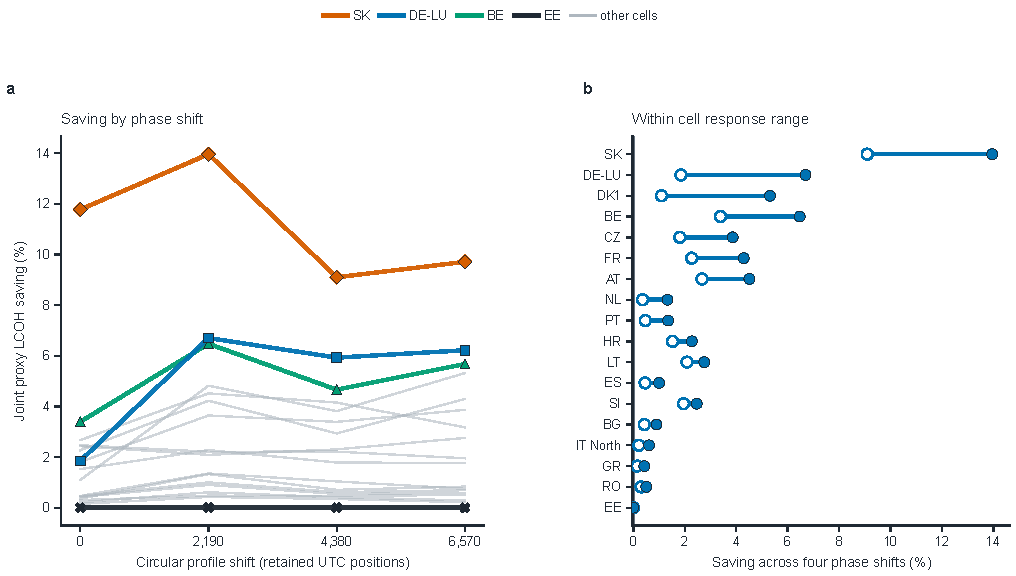
\includegraphics[width=0.97\textwidth]{figures/fig2_phase_shift_mechanism.pdf}
\refstepcounter{figure}\label{fig:phase-shift}
\end{figure}

\clearpage
\begin{figure}[p]
\centering
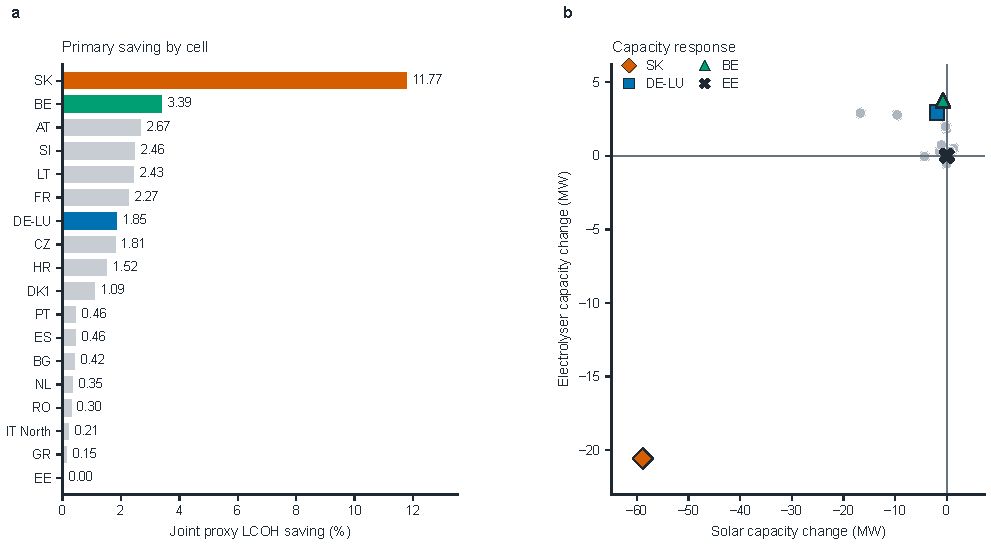
\includegraphics[width=0.97\textwidth]{figures/fig1_primary_capacity_response.pdf}
\refstepcounter{figure}\label{fig:primary-capacity}
\end{figure}

\clearpage
\begin{figure}[p]
\centering
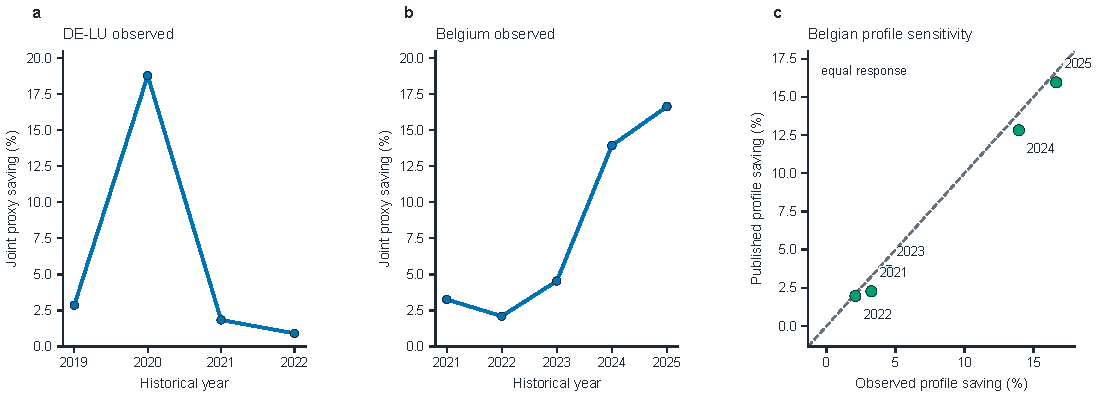
\includegraphics[width=0.97\textwidth]{figures/fig3_cross_period_profile_sensitivity.pdf}
\refstepcounter{figure}\label{fig:cross-period}
\end{figure}

\clearpage
\begin{figure}[p]
\centering
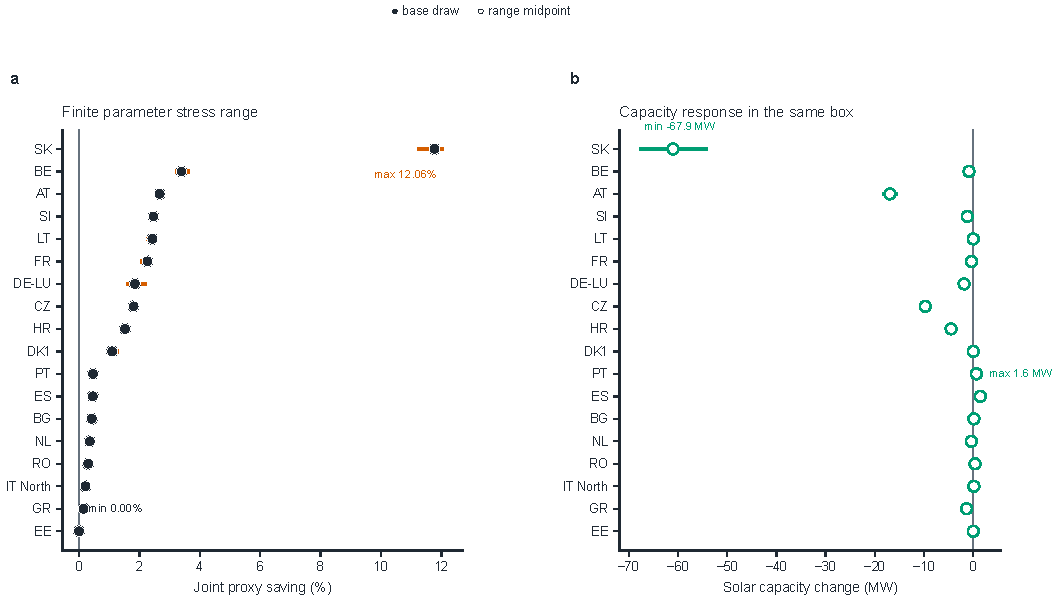
\includegraphics[width=0.97\textwidth]{figures/fig4_parameter_stress_ranges.pdf}
\refstepcounter{figure}\label{fig:parameter-stress}
\end{figure}

\clearpage
\section*{Figure captions}
\noindent\textbf{Figure 1.} Temporal coincidence mechanism (E1). Prices and trigger counts are fixed while renewable profiles rotate; the within cell saving range has a median of 0.82 percentage points and reaches 4.86 points, showing the role of temporal alignment within the model. The zero shift point reproduces the primary screen reported in Table 3. Open and filled endpoints in panel b denote the minimum and maximum phase shift responses.\par
\noindent\textbf{Figure 2.} Primary screen: LCOH savings and capacity substitutions across 18 selected cells. SK reaches 11.77\% saving with -58.8 MW solar and -20.6 MW electrolyzer capacity; EE shows zero response under the declared model boundary.\par
\noindent\textbf{Figure 3.} Cross period sensitivity (E2). Joint savings range from 0.90\% to 18.78\% across 14 retained source year/profile cells; branch attribution varies by year.\par
\noindent\textbf{Figure 4.} Bounded parameter stress (E3). The finite engineering box yields full minimum to maximum response ranges from 0.00\% to 12.06\% across the selected cells; the global saving endpoints are labeled in panel a and detailed cell endpoints are reported in Table 5. Twelve zero response joint comparisons are retained alongside positive responses. The ranges are engineering bounds, not probability intervals.\par
\end{document}
